\section{Theoretical inputs to CT18
\label{sec:Theory}}

Modern global fits  determine the PDFs from 
a large number of data points ($N_\mathit{pt}\! >\! 3600$ for CT18), provided by a wide variety of experimental measurements
(39 data sets for CT18), and involving thousands of
iterations of multivariate fits, with the theoretical cross sections evaluated at NNLO.
In the CT18 fits, the $x$ dependence of the input PDFs, at the initial scale $Q_0$ equal to the pole mass of the charm quark, is parametrized by
Bernstein polynomials, multiplied by the standard $x^a$ and $(1-x)^b$ factors that determine the small-$x$ and large-$x$ asymptotics.  In these functions, there are 5-8 independent
fitting parameters for each parton flavor except strangeness; additional parameters may be determined by momentum and 
flavor sum rules or (if poorly constrained) fixed at physically reasonable values.

In the present section, we review the essential components of our theoretical setup: the goodness-of-fit function in  Sec.~\ref{sec:chi2}, 
computer programs for (N)NLO computations for various processes  in Sec.~\ref{sec:calcs}, and 
input parametric forms for the PDFs in Sec.~\ref{sec:Paramstudies}. The explicit parametric forms for the best-fit CT18 PDFs are presented in 
Appendix~\ref{sec:AppendixParam}. 

\subsection{Goodness of fit function and the covariance matrix}
\label{sec:chi2}
%
%
The CTEQ-TEA analyses quantify the goodness-of-fit to an experimental data set
$E$ with $N_{pt}$
data values by means of the log-likelihood function~\cite{Pumplin:2002vw},
%
\begin{equation}
\chi_{E}^{2}(a,\lambda)=\sum_{k=1}^{N_{pt}}\frac{1}{s_{k}^{2}}\left(D_{k}-T_{k}(a)-\sum_{\alpha=1}^{N_{\lambda}}\lambda_{\alpha}\beta_{k\alpha}\right)^{2}+\sum_{\alpha=1}^{N_{\lambda}}\lambda_{\alpha}^{2}.\label{Chi2sys}
\end{equation}
%
A $k$-th datum is typically provided as a central value $D_{k},$ an uncorrelated
statistical error $s_{k,\mbox{\scriptsize stat}}$, and possibly an
uncorrelated systematic error
$s_{k,\mbox{\scriptsize uncor sys}}$.
Then, $s_{k}\equiv \sqrt{s_{k,\mbox{\scriptsize stat}}^{2}+s_{k,\mbox{\scriptsize uncor sys}}^{2}}$
is the total uncorrelated error on the measurement $D_{k}$.

$T_{k}$ is the corresponding theory value that depends on the PDF
parameters $\left\{a_1,a_2,...\right\}\equiv a$. In addition, the $k$-th datum may depend on
$N_{\lambda}$ correlated systematic uncertainties, and those may
be fully correlated over all data points. To estimate such errors,
it is common to associate each source of the correlated error with
an independent random nuisance parameter $\lambda_{\alpha}$ that is assumed to
be sampled from a standard normal distribution, unless known
otherwise. The experiment does not tell us the values of
$\lambda_{\alpha}$
but it may provide
the change $\beta_{k\alpha}\lambda_\alpha$ of $D_k$ under a variation of $\lambda_{\alpha}$. Knowing $\beta_{k\alpha}$,
one can estimate the likely values of $\lambda_{\alpha}$, as well
as the uncertainty in the PDF parameters for a plausible range of
$\lambda_{\alpha}$.


For those experiments $E$ that provide
$\beta_{k\alpha}$, we find that, at the global minimum $a_0$,
the best-fit $\chi^2$ value is given as
\begin{equation}
\chi^{2}_E (a_{0},\overline \lambda(a_0))=
\sum_{i=1}^{N_{pt}} r_i^2(a_0)
+\sum_{\alpha=1}^{N_\lambda}\overline\lambda^2_\alpha(a_0) \label{Chi2a0l0}
\end{equation}
in terms of the best-fit {\it shifted residuals},
%
\begin{equation}
  r_{i}(a_0)\  =\ s_{i}\sum_{j=1}^{N_{\mathit{pt}}}(\mathrm{cov}^{-1})_{ij}\,\left(D_{j}-T_{j}(a_0)\right),\label{eq:res-cov}
\end{equation}
and best-fit nuisance parameters,
\begin{equation}
\overline{\lambda}_{\alpha}(a_0) =\sum_{i,j=1}^{N_{\mathit{pt}}}(\mathrm{cov}^{-1})_{ij}\frac{\beta_{i\alpha}}{s_{i}}\frac{\left(D_{j}-T_{j}(a_0)\right)}{s_{j}},
\label{eq:lam-cov}
\end{equation}
%
where
%
\begin{equation}
(\mathrm{cov}^{-1})_{ij}\ =\ \left[\frac{\delta_{ij}}{s_{i}^{2}}\,-\,\sum_{\alpha,\beta=1}^{N_{\lambda}}\frac{\beta_{i\alpha}}{s_{i}^{2}}A_{\alpha\beta}^{-1}\frac{\beta_{j\beta}}{s_{j}^{2}}\right]\ ,\label{eq:covmat}
\end{equation}
%
and
%
\begin{equation}
A_{\alpha\beta}\ =\ \delta_{\alpha\beta}\,+\,\sum_{k=1}^{N_{\mathit{pt}}}\frac{\beta_{k\alpha}\beta_{k\beta}}{s_{k}^{2}}\ .
\end{equation}
These relations are derived in Appendix~\ref{sec:chi2_app}.

Another instructive form expresses $r_i(a_0)$ in terms of the
shifted data values, $D_i^{sh}\equiv D_i -
\sum_{\alpha=1}^{N_{\lambda}}\overline \lambda_{\alpha}(a_0) \beta_{k\alpha}$:
\begin{equation}
r_{i}(a_0) = \frac{D_{i}^{sh}(a_0)-T_{i}(a_0)}{s_{i}}. \label{riShifted}
\end{equation}

Sometimes, we take extra steps to
convert the published table of correlated
uncertainties into the $\beta_{k\alpha}$ matrix formatted in accord
with Eq.~(\ref{Chi2sys}).
For example, when an experiment distinguishes between positive
and negative systematic variations, we average these for each data
point for consistency with the normally distributed $\lambda_{\alpha}$.
{[}We have verified that the choice of the averaging procedure
does not significantly affect the
outcomes, {\it e.g.}, if a central value is shifted to be in the middle of an originally
asymmetric interval, {\it etc.}{]}

In a small number of  experimental publications, only
a form based on the covariance
matrix $\left(\mbox{cov}\right)_{ij}$ is used in place of Eq.~(\ref{Chi2sys}):
\begin{equation}
\chi_{E}^{2}(a)=\sum_{i,j=1}^{N_{pt}}\left(\mbox{\mbox{cov}}^{-1}\right)_{ij}\left(D_{i}-T_{i}(a)\right)\left(D_{j}-T_{j}(a)\right).\label{Chi2CovMat1}
\end{equation}
While we can compute $\chi^2$ directly using
Eq.~(\ref{Chi2CovMat1}), when deriving the PDFs, we find it convenient
to go back to the form consisting of the uncorrelated errors $s_i$ and
the correlated contributions provided by $\beta_{k\alpha}$:
\begin{equation}
  (\mbox{cov})_{ij} \approx s_i^2 \delta_{ij}
  +\sum_{\alpha=1}^{N_\lambda} \beta_{i\alpha}\beta_{j\alpha}.\label{covapprox}
\end{equation}
An algorithm to construct such a representation with sufficient
accuracy is presented at the end of Appendix~\ref{sec:chi2_app}. In
all relevant cases, we have checked that both the input covariance matrix
$(\mbox{cov})_{ij}$ and its decomposed version (\ref{covapprox})
produce close values of $\chi^2$. With the latter representation, we
are also able to examine the shifted data values and shifted
residuals, Eq.~(\ref{riShifted}), to explore agreement with the
individual data points. 

In this article, we generally follow the CTEQ methodology and obtain
$r_{i}(a_0)$ directly from the CTEQ-TEA fitting program, together
with the optimal nuisance parameters $\overline{\lambda}_{\alpha}(a_0)$
and shifted central data values $D_{i}^{sh}(a).$
%-  -  -  -  -  -  -  -  -  -  -  -  -  -  -  -  -  -  -  -  -  -  -  -  -  -  -  -  -  -  -  -  -  -

\subsection{Theoretical computations and programs \label{sec:calcs}}
\subsubsection{Overview
\label{sec:TheorySettings}}
%
%

For deep-inelastic scattering observables, we perform computations using an NNLO realization \cite{Guzzi:2011ew} of the SACOT-$\chi$ heavy-quark scheme \cite{Aivazis:1993pi,Aivazis:1993kh,Kramer:2000hn,Tung:2001mv} adopted since CT10 NNLO \cite{Gao:2013xoa}. These can be done using either the pole or $\overline{\mathrm{MS}}$ quark masses as the input \cite{Gao:2013wwa}, with the default choices of quark masses set to be $m_c^{pole}=1.3$ GeV in CT18, A, and X ($m_c^{pole}=1.4$ GeV in CT18Z), and $m_b^{pole}=4.75$ GeV.  The neutral-current DIS cross sections are evaluated at NNLO directly in the fitting code. For charged-current DIS cross sections,  the NNLO cross sections from heavy quarks can be obtained by fast interpolations with pre-generated grids based on the calculation presented in Ref.~\cite{Berger:2016inr}. The impact of the NNLO contribution on the description of the charged-current dimuon DIS data is further discussed in Sec.~\ref{sec:Qualitydimuon}.

The computational complexity of NNLO matrix elements precludes their direct evaluation for each fit iteration, particularly given the expansive size of the data sets fitted in CT18. Instead, for the
newly included high-precision data from the LHC, \texttt{ApplGrid}~\cite{Carli:2010rw} and \texttt{fastNLO}~\cite{Wobisch:2011ij} 
fast tables have been generated using programs such as \texttt{MCFM}~\cite{Campbell:2010ff}, \texttt{NLOJet++}~\cite{Nagy:2003tz} and 
\texttt{aMCfast}~\cite{Bertone:2014zva}, to allow fast evaluation of the matrix elements as the PDF parameters are varied. 
NNLO cross sections are then evaluated using NNLO/NLO point-by-point $K$-factors determined using the fast tables and NNLO programs such 
as \texttt{NNLOJET}~\cite{Buza:1997mg,Ridder:2015dxa,Gehrmann-DeRidder:2017mvr,Currie:2016bfm,Currie:2017ctp}, \texttt{FEWZ}~\cite{Gavin:2010az,Gavin:2012sy,Li:2012wna}, 
\texttt{MCFM}~\cite{Campbell:2010ff,Boughezal:2016wmq,MCFM8} and \texttt{DYNNLO}~\cite{Catani:2007vq,Catani:2009sm}. 
One exception is the top-quark data from ATLAS and CMS, for which \texttt{fastNNLO} tables have been 
provided by the authors for the NNLO cross sections~\cite{Czakon:2016dgf,Czakon:2018nun}. The programs used for the calculation of the cross sections for each data set are summarized 
in Table~\ref{Theory-Calc-II}. 

\begin{table}[b]
\begin{tabular}{|c|c|c|c|c|c|c| }
\hline
ID\# & Process   &   Expt.   & fast table  & NLO code &  NNLO $K$-factors  & $\mu_{R,F}$\\
\hline
245  & \multirow{5}{*}{$W/Z$}  & LHCb7WZ    & \multirow{5}{*}{\texttt{APPLgrid}}   & \multirow{5}{*}{\texttt{MCFM/aMCfast}}   & \multirow{2}{*}{\texttt{FEWZ/MCFM}}   &  \multirow{5}{*}{$M_{W,Z}$}  \\
246  &  & LHCb8Zee    &  &  &  &  \\
248  &  & ATL7WZ   &  &  & \texttt{FEWZ/MCFM/DYNNLO}  &  \\
249  &  & CMS8Wasy   &  &  & \multirow{2}{*}{\texttt{FEWZ/MCFM}} &  \\
250  &  & LHCb8WZ   &  &  &  &  \\
\hline
253 & $Z+{\rm jet}$  & ATL8ZpT   & \texttt{APPLgrid} &  \texttt{MCFM} & \texttt{NNLOJET}  & $\sqrt{(p_{T}^{ll})^{2}+M_{ll}^{2}}$ \\
\hline
542 &\multirow{3}{*}{Incl. jet} & CMS7jets   & \texttt{fastNLO}  & \multirow{3}{*}{  \texttt{NLOJet++} }  & \multirow{3}{*}{ \texttt{NNLOJET}}   &  \multirow{ 3}{*}{$p_{T}$}    \\
544 &  &  ATL7jets & \texttt{APPLgrid} & & &  \\
545 &  & CMS8jets   & \texttt{fastNLO}  &  &   &      \\  
\hline
573 & \multirow{2}{*}{$t\bar{t}$} &  CMS8ttb  &
\multicolumn{3}{|c|}{\multirow{2}{*}{\texttt{fastNNLO} }  } &
\multirow{2}{*}{ $\frac{H_{T}}{4}$, $\frac{m_{T}}{2}$}\\
580 &   &   ATL8ttb & \multicolumn{3}{|c|}{} & \\
\hline
\end{tabular}
\caption{Theory calculations for the high-precision data from the LHC which are newly included in the CT18(Z) global fit. 
The $K$-factors of ATL7WZ (ID 248) extracted from \texttt{xFitter} are calculated with \texttt{DYNNLO} 
and compared with \texttt{FEWZ} and \texttt{MCFM} in App. \ref{sec:Appendix4xFitter}. 
\label{Theory-Calc-II}}
\end{table}


Because of non-negligible statistical errors due to Monte-Carlo (MC) integration in the NNLO calculations, it was necessary to fit the $K$-factors with smooth curves and add a
small {\it MC error} (in this analysis, equal to $0.5\%$ of the data) to the calculations for the high-$p_T$ $Z$ and inclusive jet production processes, as specified below.

For the legacy data on electroweak boson production, already included in the CT14 and \CTHERAII, 
we inherit the original CTEQ calculations summarized in Table~\ref{Theory-Calc-VB}. 
The NLO calculation is directly performed by the CT fitting code, while the point-by-point $K$-factors are calculated with 
\texttt{Vrap}~\cite{Anastasiou:2003ds,Anastasiou:2003yy}, \texttt{ResBos}~\cite{Ladinsky:1993zn,Konychev:2005iy} and
\texttt{FEWZ}~\cite{Gavin:2010az,Gavin:2012sy,Li:2012wna}.

\begin{table}[tb]
\begin{tabular}{|c|c|c|c|c|c| }
\hline
ID\# & Obs.   &   Expt.   &  NLO code &  NNLO $K$-factors  & $\mu_{R,F}$\\
\hline
%245  & $y_{\mu\mu},\eta_{\mu}$  & LHCb7ZW 
 %  & \multirow{4}{*}{\texttt{APPLgrid}} & \multirow{4}{*}{\texttt{MCFM/aMCfast} }& \multirow{4}{*}{\texttt{MCFM/FEWZ} }  & \multirow{4}{*}{$M_{Z,W}$}  \\
%246  & $y_{ee}$   & LHCb8Z &  &   &  &    \\
%250 & $y_{\mu\mu},\eta_{\mu}$  &  LHCb8ZW &  &   &  &   \\
%249 &  $A(\mu)$  & CMS8W  &  &   &  &  \\
%\hline
%253 &  $p_{T}^{ll}$  &  ATL8Z & \texttt{APPLgrid}  & \texttt{MCFM}  & \texttt{NNLOJet}  &  $M_{T}^{ll}$\\
%\hline
201 & $\sqrt{\tau}, y$  &  E605  &  \multirow{3}{*}{ \texttt{CTEQ}}  & \multirow{3}{*}{ \texttt{FEWZ}  }   & \multirow{3}{*}{$Q_{ll}$} \\
203  & $\sigma_{pd}/\sigma_{pp},x_{F}$  & E866rat &  &    & \\
204  & $Q,x_{F}$ &  E866pp  &  &    & \\
\hline
225 & $A(e)$  & CDF1Z  &  \multirow{4}{*}{ \texttt{CTEQ}}  &  \multirow{4}{*}{ \texttt{ResBos}}  &  $Q_{ll}$   \\
227 & $A(e)$  &CDF2W &     &  &  \multirow{3}{*}{$M_{W}$} \\
234 &  $A(\mu)$ & D$\varnothing$2W &    && \\
281 & $A(e)$  & D$\varnothing$2W  &   &&  \\
\hline
260 &  $y_{ll}$ &  D$\varnothing$2Z &   \multirow{2}{*}{ \texttt{CTEQ}}  &  \multirow{2}{*}{\texttt{Vrap}}  &
\multirow{2}{*}{ $Q_{ll}$ } \\
261 &  $y_{ll}$ &  CDF2Z  &      &  &\\
\hline 
266 & $A(\mu)$  & CMS7W  &   \multirow{3}{*}{\texttt{CTEQ} }  &\multirow{3}{*}{ \texttt{ResBos}} & \multirow{2}{*}{ $M_{W}$}   \\
267  & $A(e)$  & CMS7W  &        &  &\\
268 &  $y_{ll},\eta_{l},A(l)$   & ATL7WZ12  &   &   & $M_{Z,W}$ \\
\hline
%248 &  $y_{ll},\eta_{l}$  &  ATL7ZW{\tiny(2016)} &   \texttt{APPLgrid}  & \texttt{MCFM/aMCfast}  & \texttt{MCFM/FEWZ}  &  $M_{Z,W}$\\
%\hline 
\end{tabular}
\caption{Theory calculations for the CT14 and \CTHERAII's legacy data of electroweak vector boson production.
\label{Theory-Calc-VB}}
\end{table}

Even with the use of stored grids for fast evaluation of the matrix
elements, significant improvements on speed are needed. The CT fitting
code has been upgraded to a multi-threaded version with a two-layer
parallelization, through a rearrangement of the minimization
algorithm and via a redistribution of the data sets. As a result, the speed of calculations increased by up to a factor of 10. Details are provided in
Appendix~\ref{sec:AppendixCodeDevelopment}.  

We will now describe the theoretical calculations for each new LHC process included in the CT18(Z) fits.
% ~ ~ ~ ~ ~ ~ ~ ~ ~ ~ ~ ~ ~ ~ ~ ~ ~ ~ ~ ~
%

\subsubsection{LHC inclusive jet data
\label{sec:TheoryJets}
}

LHC inclusive jet data are available with different jet radii. We have chosen the larger of the two nominal jet radii, 
0.6 for ATLAS and 0.7 for CMS, to reduce dependence on resummation/showering and hadronization effects~\cite{Bellm:2019yyh}. 
There is a non-negligible difference at low jet transverse momentum between theory predictions at NNLO 
using as the momentum-scale choice of either the inclusive jet $p_T$ or the leading jet $p_T$ ($p_{T1}$)~\cite{Currie:2018xkj} .
The nominal choice adopted by the CTEQ-TEA group is to use the inclusive jet $p_T$. 
We have observed that the fitted gluon PDF is not very sensitive to this choice even in the kinematic regions 
where the difference in NNLO predictions between these two scale choices is important.
%This resilience in the global fit is due both to the presence of other data in the relevant kinematic regions, and to QCD evolution.
%

Electroweak corrections from Ref.~\cite{Dittmaier:2012kx} were applied
to jet cross sections and can be as large as 10\% for the highest transverse momentum bin in the central
rapidity region, but decrease quickly with increasing rapidity and with decreasing jet transverse momentum.
Furthermore, the QCD NNLO/NLO $K$-factors were fitted with smooth curves, and a 0.5\% theoretical error
assessed with respect to the data has been added to each data value to take into account the fluctuations
in integration of NNLO cross sections provided by \texttt{NNLOJET}.  


% ~ ~ ~ ~ ~ ~ ~ ~ ~ ~ ~ ~ ~ ~ ~ ~ ~ ~ ~ ~
%
\subsubsection{LHC electroweak gauge boson hadroproduction}
%
%In what follows we give a brief description of the Drell-Yan theory calculations at NNLO
%used in the CT18($Z$) global analysis.
The Drell-Yan theory calculations at NNLO in the CT18(Z) global analysis consist of the following:

\begin{itemize}
\item ATLAS 7 TeV 4.6 fb$^{-1}$ measurements of $W^{\pm}$ and $Z/\gamma^{*}$ production cross 
sections in the $e$ and $\mu$ decay channels~\cite{Aaboud:2016btc}: 
the theory predictions at NLO are obtained by using \texttt{APPLgrid}~\cite{Carli:2010rw} fast tables 
generated with \texttt{MCFM}~\cite{Campbell:2010ff} and validated against \texttt{aMCfast}~\cite{Bertone:2014zva} 
interfaced with \texttt{MadGraph5\_aMC@NLO}~\cite{Alwall:2014hca}. The NNLO corrections are imported from the 
\texttt{xFitter}~\cite{Alekhin:2014irh} analysis published in Ref.~\cite{Aaboud:2016btc}. These corrections are 
obtained using the \texttt{DYNNLO-1.5} code  \cite{Catani:2007vq,Catani:2009sm}, and checked against  \texttt{FEWZ-3.1.b2}~\cite{Gavin:2010az,Gavin:2012sy,Li:2012wna} and \texttt{MCFM-8.0} \cite{Boughezal:2016wmq} codes. Some discrepancy among these codes (up to $\sim\!1\%$) were found. However,  
these discrepancies do not induce significant differences
in the calculated results like $\chi^2$. More details can be found in Appendix~\ref{sec:Appendix4xFitter}.


\item CMS 8 TeV 
$18.8 \mbox{ fb}^{-1}$ measurements of muon charge asymmetry~\cite{Khachatryan:2016pev}: 
The theory predictions at NLO are from \texttt{APPLgrid} generated with \texttt{MCFM}, while for the NNLO 
corrections, we use $K$-factors calculated with \texttt{FEWZ-3.1}. These predictions have also been validated with \texttt{MCFM-8.0}. 

\item LHCb 7 TeV $W/Z$ cross sections, $W$ charge asymmetry measurements with 1 fb$^{-1}$ of integrated luminosity~\cite{Aaij:2015gna}, 
and LHCb 8 TeV measurements including both the electron \cite{Aaij:2015vua} and muon \cite{Aaij:2015zlq} channels: 
the NLO theory calculation is obtained by using \texttt{APPLgrid} fast tables generated with \texttt{MCFM}. 
These have been validated against \texttt{MadGraph5\_aMC@NLO} + \texttt{aMCfast}. The NNLO corrections are calculated with  \texttt{FEWZ}, and validated by \texttt{MCFM}.

\item ATLAS~\cite{Aad:2014xaa,Aad:2015auj} and CMS~\cite{Khachatryan:2015oaa} measurements of transverse momentum of Drell-Yan lepton pairs at 7 TeV and/or 8 TeV. 
The CT18(Z) fit includes only the ATLAS 8 TeV absolute differential cross section measurements. The NLO theoretical calculation is performed with \texttt{APPLgrid} generated with \texttt{MCFM}. The NNLO corrections are provided by the \texttt{NNLOJET} group \cite{Ridder:2015dxa,Gehrmann-DeRidder:2017mvr}.
We have fitted the NNLO/NLO $K$-factors with smooth curves and include a 0.5\% MC error to account for the fluctuations in the NNLO calculations.
In addition, we have imposed the kinematic cut $45\!<\!p_{T}^{ll}\!<\!150$ GeV  to ensure reliability of the fixed-order calculation. 
The low-$p_{T}^{ll}$ region is dropped due to the non-negligible contribution from QCD soft-gluon resummation, and the high $p_{T}^{ll}$ region is dropped because the EW corrections there are expected to grow~\cite{Hollik:2015pja,Kallweit:2015fta}.
%
%
%
%The CMS 8 TeV $Z$ $p_{T}$ measurements are not included in the CT18(Z) analysis as they are less inclusive. The NLO theory prediction is obtained by using \texttt{APPLgrid} generated with \texttt{MCFM}. The NNLO corrections were provided by the \texttt{NNLOjet} group \cite{Gehrmann-DeRidder:2017mvr}. A 0.5\%  uncorrelated error is included to account for the MC uncertainty in the NNLO calculation. Factorization and renormalization scales are set to $\mu_{R}=\mu_{F}=\sqrt{p_{T}^{2}+M_{ll}^{2}}$, where the $M_{ll}$ is the invariant mass of the lepton pair. We have explored the scale dependence of the theoretical predictions for this data, with the choice of $\sqrt{p^2_T + M^2_{ll}}$ appearing satisfactory.

\end{itemize}

\subsubsection{Top-quark pair production
\label{sec:TheoryTop}
}
%
Theory predictions for top-quark pair production differential distributions at the LHC 8 TeV are implemented at NNLO in QCD using
\texttt{fastNNLO} tables~\cite{Czakon:2017dip,fastnnlo:grids}. 
In the CT18 global fit, the top-quark mass has been set to $m_t^{\rm pole}=173.3$ GeV. Motivated by~\cite{Czakon:2016dgf}, we chose the default central scale
$\mu_{F,R}\equiv \mu =1/2\sqrt{m_t^2 + p_{T,t}^2}$ for the top-quark $p_T$ spectrum, while the rest of the distributions are obtained with
$\mu=1/4\left(\sqrt{m_t^2 + p_{T,t}^2} + \sqrt{m_t^2 + p_{T,\bar{t}}^2}\right)$.
The impact of the EW corrections on the theory predictions for $t \bar{t}$ differential distributions has been studied in~\cite{Czakon:2017wor} 
where the difference between the additive and
multiplicative approaches for combining QCD and EW corrections is also investigated. EW $K$-factors 
from an analytic fit for the QCD $\times$ EW/QCD contributions are  available~\cite{EW:kfac}. 
The CT18 global analysis does not include EW corrections in $\bar{t} t$ production. Their impact on the fitted PDFs is expected to be small in the kinematic range of the differential distributions currently considered.   

The impact of the EW corrections on the CT18 theory predictions at CMS 13 TeV is illustrated in Sec.~\ref{sec:StandardCandles}. In this case, the CT18 theory predictions include EW corrections evaluated using the multiplicative approach of~\cite{Czakon:2017wor}, and the recommended value of $m_t^{\rm pole}=172.5$ GeV has been used to compare theory and the CMS data (without fitting the data).

\subsection{The nonperturbative parametrization form} 
\label{sec:Paramstudies}

An important source of the uncertainty in the CTEQ PDF analysis is associated with the choice of the parametric form for the fitted distributions at the lower boundary of QCD evolution, $f_a(x,\Q\! =\! Q_0)$. There is limited guidance
from theory as to the most appropriate PDF parametrizations, and it is
favorable to guarantee a maximal level of parametric flexibility without
overfitting experimental data~\cite{Kovarik:2019xvh}. In App.~\ref{sec:AppendixParam}, we present the explicit parametrization forms used in CT18. As usual, the PDFs at higher scales $Q>Q_0$ are computed
using the Dokshitser-Gribov-Lipatov-Altarelli-Parisi (DGLAP) equations at NNLO, with splitting kernels available from Refs.~\cite{Moch:2004pa,Vogt:2004mw,Ablinger:2014nga,Ablinger:2017tan}.
%
%

To estimate the parametrization dependence, we repeated the CT fits multiple times using a large number (more than 100) of initial parametrization forms which have comparable numbers of fitting
parameters. The final PDFs are obtained using a fixed parametrization form, but the uncertainty is computed so as to cover the bulk of the solutions obtained with the alternative parametrizations.  The results of this study are illustrated in Fig.~\ref{fig:params},
which show central fits for a range of alternative fitting forms (green curves) superposed within
the uncertainty band (at the 90\% confidence level) for an early version of CT18. 
%
%

As we increased the number of free PDF parameters, an improvement in the global $\chi^2$ or individual $S_E$ values was typically found, so long as $\lesssim\! 30$ free parameters were fitted. With more than about 30 parameters, the fits tend
to destabilize, as expanded parametrizations attempt to describe statistical noise.
The final PDFs are based on the parametrizations with a total of 29 free parameters. For each of the four fits, we provide twice as many Hessian error PDFs to evaluate the PDF uncertainties according to the CTEQ6 master formulas \cite{Pumplin:2002vw}.

\begin{figure}[tb]
        \center
	\hspace*{-0.5cm}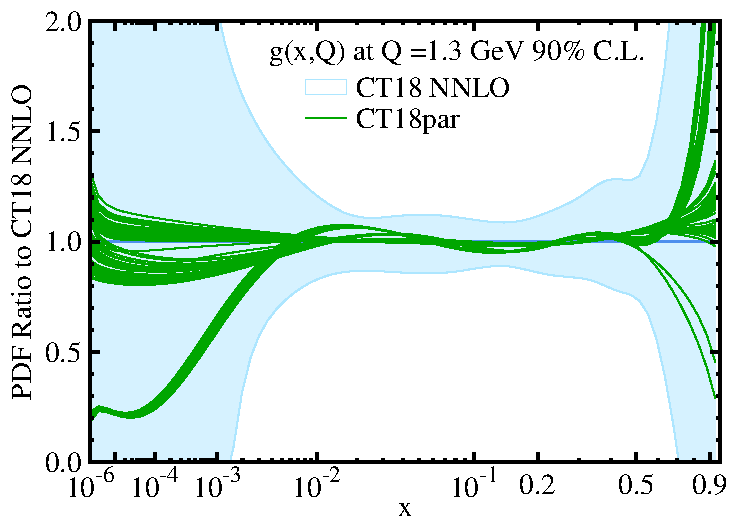
\includegraphics[width=0.51\textwidth]{fig/params/g_par_CT18_ect.pdf}
        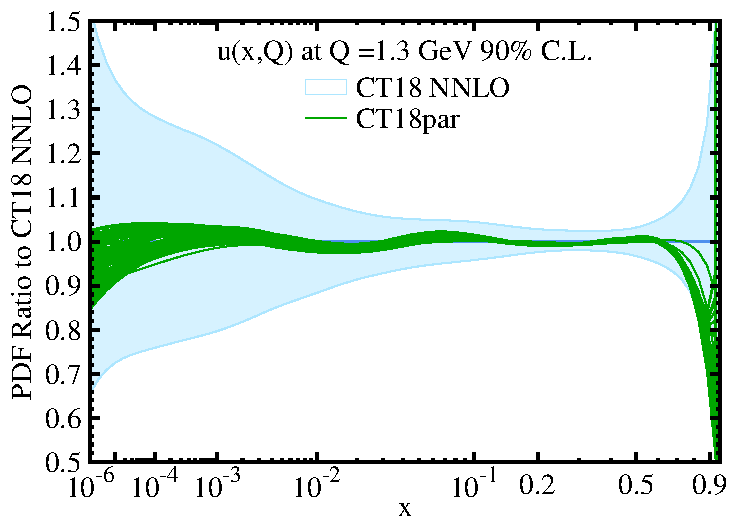
\includegraphics[width=0.51\textwidth]{fig/params/u_par_CT18_ect.pdf}\\
        \hspace*{-0.5cm}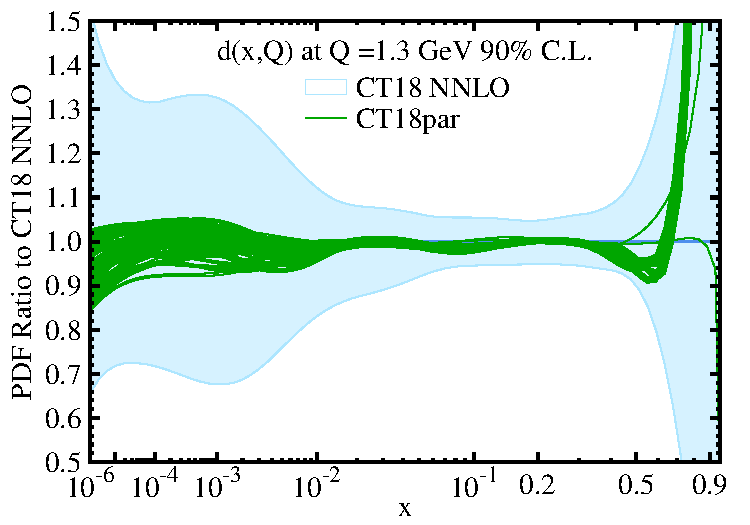
\includegraphics[width=0.51\textwidth]{fig/params/d_par_CT18_ect.pdf}
        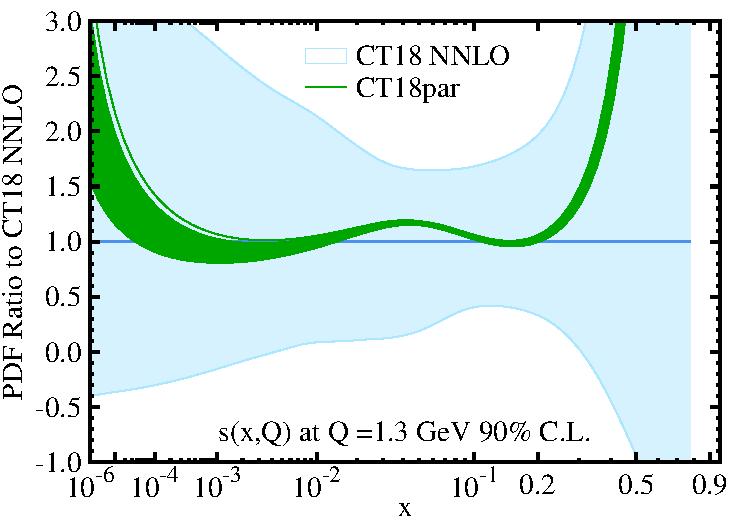
\includegraphics[width=0.51\textwidth]{fig/params/s_par_CT18_ect.pdf}\\
        \hspace*{-0.5cm}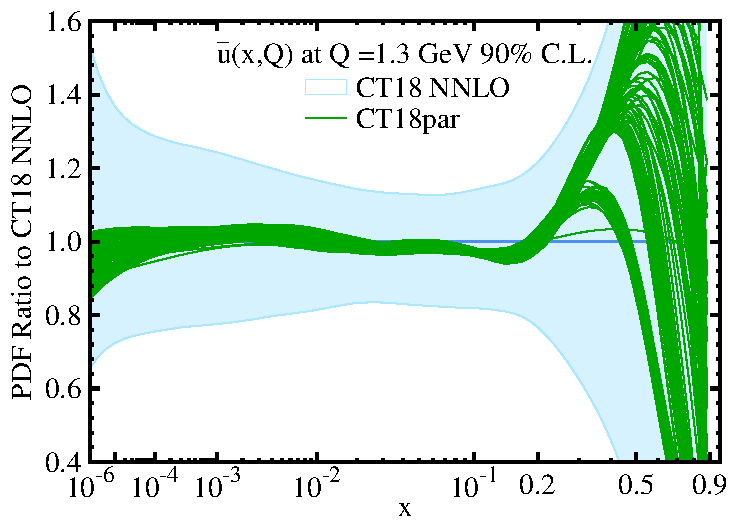
\includegraphics[width=0.51\textwidth]{fig/params/ubar_par_CT18_ect.pdf} 
        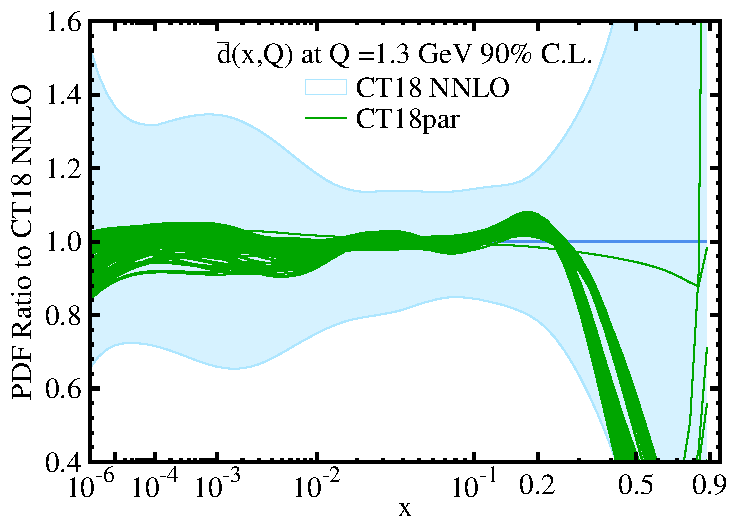
\includegraphics[width=0.51\textwidth]{fig/params/dbar_par_CT18_ect.pdf}
        \caption{
	To understand the parametrization dependence in the CT18 fit, we performed $\mathcal{O}(100)$ candidate
	PDF analyses using a wide range of alternative functional forms for $f_a(x,Q_0)$. The green curves
	in the panels above illustrate the spread of central fits achieved with the various candidate fits,
	evaluated as ratios with respect to the central CT18 fit.
		}
\label{fig:params}
\end{figure}
\clearpage
